\chapter{Retrieval Stability in High Dimensions}
\label{chapter:instability}

\abstract{
We are about to embark on a comprehensive survey and analysis of vector retrieval methods
in the remainder of this monograph. It may thus sound odd to suggest that you may not need
any of these clever ideas in order to perform vector retrieval.
Sometimes, under bizarrely general conditions that we will explore formally in this chapter,
an exhaustive search (where we compute the distance between query and every data point,
sort, and return the top $k$) is likely to perform much better in both accuracy and search latency!
The reason why that may be the case has to do with the approximate nature of algorithms
and the oddities of high dimensions. We elaborate this point by focusing on the top-$1$
case.}

\section{Intuition}
\label{chapter:instability:stability:intuition}
Consider the case of proper distance functions where $\delta(\cdot, \cdot)$ is a metric.
Recall from Equation~(\ref{equation:flavors:approximate-top-k-retrieval}) that a vector
$u$ is an acceptable $\epsilon$-approximate solution if its distance to the query $q$ according to $\delta(\cdot, \cdot)$
is at most $(1 + \epsilon) \delta(q, u^\ast)$, where $u^\ast$ is the optimal vector
and $\epsilon$ is an arbitrary parameter.
As shown in Figure~\subref*{figure:flavors:flavors:approximate-knn} for NN,
this means that, if you centered an $L_p$ ball around $q$ with
radius $\delta(q, (1 + \epsilon) u^\ast)$, then $u$ is in that ball.

So, what if we find ourselves in a situation where no matter how small $\epsilon$ is,
too many vectors, or indeed \emph{all} vectors, from our collection $\mathcal{X}$ end up
in the $(1+\epsilon)$-enlarged ball? Then, by definition, every vector is an $\epsilon$-approximate nearest neighbor of $q$!

In such a configuration of points,
it is questionable whether the notion of ``nearest neighbor'' has any meaning at all:
If the query point were perturbed by some noise as small as $\epsilon$,
then its true nearest neighbor would suddenly change, making NN \emph{unstable}.
Because of that instability, any approximate algorithm will need to examine a large portion or nearly all
of the data points anyway, reducing thereby to a procedure that performs
more poorly than exhaustive search.

That sounds troubling. But when might we experience that phenomenon? That is the
question~\cite{beyer1999nnMeaningful} investigate in their seminal paper.

\begin{svgraybox}
It turns out, one scenario where vector retrieval becomes unstable as dimensionality $d$ increases is
if a) data points are \emph{iid} in each dimension,
b) query points are similarly drawn \emph{iid} in each dimension, and
c) query points are independent of data points. This includes many
synthetic collections that are, even today, routinely but inappropriately used
for evaluation purposes.
\end{svgraybox}

On the other hand, when data points form clusters and query points
fall into these same clusters, then the (approximate) ``nearest cluster''
problem is meaningful---but not necessarily the approximate NN problem.
So while it makes sense to use approximate algorithms to obtain the nearest
cluster, search within clusters may as well be exhaustive.
This, as we will learn in Chapter~\ref{chapter:ivf},
is the basis for a popular and effective class of vector retrieval
algorithms on real collections.

\section{Formal Results}
More generally, vector retrieval becomes unstable in high dimensions
when the variance of the distance between query and data
points grows substantially more slowly than its expected value.
That makes sense. Intuitively, that means that more and more data points
fall into the $(1 + \epsilon)$-enlarged ball centered at the query.
This can be stated formally as the following theorem due to~\cite{beyer1999nnMeaningful},
extended to any general distance function $\delta(\cdot, \cdot)$.

\begin{theorem}
\label{theorem:instability:beyer}
    Suppose $m$ data points $\mathcal{X} \subset \mathbb{R}^d$ are drawn iid from a data distribution
    and a query point $q$ is drawn independent of data points from any distribution.
    Denote by $X$ a random data point. If
    \begin{equation*}
        \lim_{d \rightarrow \infty} \var\big[ \delta(q, X) \big] / \ev\big[ \delta(q, X) \big]^2 = 0,
    \end{equation*}
    then for any $\epsilon > 0$,
    $\lim_{d \rightarrow \infty} \probability\big[ \delta(q, X) \leq (1 + \epsilon) \delta(q, u^\ast) \big] = 1,$
    where $u^\ast$ is the vector closest to $q$.
\end{theorem}
\begin{proof}
    Let $\delta_\ast = \max_{u \in \mathcal{X}} \delta(q, u)$ and $\delta^\ast = \min_{u \in \mathcal{X}} \delta(q, u)$.
    If we could show that, for some $d$-dependent \emph{positive} $\alpha$ and $\beta$ such that $\beta/\alpha = 1 + \epsilon$,
    $\lim_{d \rightarrow \infty} \probability\big[ \alpha \leq \delta^\ast \leq \delta_\ast \leq \beta \big] = 1$,
    then we are done. That is because, in that case $\delta_\ast/\delta^\ast \leq \beta / \alpha = 1 + \epsilon$ almost surely
    and the claim follows.
    
    From the above, all that we need to do is to find $\alpha$ and $\beta$ for a given $d$.
    Intuitively, we want the interval $[\alpha, \beta]$ to contain $\ev[\delta(q, X)]$, because
    we know from the condition of the theorem that the distances should concentrate around their mean.
    So $\alpha = (1 - \eta) \ev[\delta(q, X)]$ and $\beta = (1 + \eta) \ev[\delta(q, X)]$ for some $\eta$
    seems like a reasonable choice. Letting $\eta = \epsilon / (\epsilon + 2)$ gives us the desired ratio:
    $\beta/\alpha = 1 + \epsilon$.
    
    Now we must show that $\delta_\ast$ and $\delta^\ast$ belong to our
    chosen $[\alpha, \beta]$ interval almost surely in the limit. That happens if \emph{all} distances belong to 
    that interval. So:
    \begin{align*}
        \lim_{d \rightarrow \infty} &\probability\big[ \alpha \leq \delta^\ast \leq \delta_\ast \leq \beta \big] = \\
        &\lim_{d \rightarrow \infty} \probability\Big[ \delta(q, u) \in [\alpha, \beta] \quad \forall \; u \in \mathcal{X} \Big] = \\
        &\lim_{d \rightarrow \infty} \probability\Big[ (1 - \eta) \ev[\delta(q, X)] \leq \delta(q, u) \leq (1 + \eta) \ev[\delta(q, X)] \; \forall \; u \in \mathcal{X} \Big] = \\
        &\lim_{d \rightarrow \infty} \probability\Big[ \big\lvert \delta(q, u) - \ev[\delta(q, X)] \big\rvert \leq \eta \ev[\delta(q, X)] \quad \forall \; u \in \mathcal{X} \Big].
    \end{align*}
    It is now easier to work with the complementary event:
    \begin{equation*}
        1 - \lim_{d \rightarrow \infty} \probability\Big[ \exists \; u \in \mathcal{X} \; \mathit{s.t.} \quad \big\lvert \delta(q, u) - \ev[\delta(q, X)] \big\rvert > \eta \ev[\delta(q, X)] \Big].
    \end{equation*}
    Using the Union Bound, the probability above is greater than or equal to the following:
    \begin{align*}
    \lim_{d \rightarrow \infty} &\probability\big[ \alpha \leq \delta^\ast \leq \delta_\ast \leq \beta \big] \geq \\
        &1 - \lim_{d \rightarrow \infty} \sum_{u \in \mathcal{X}} \probability\Big[\big\lvert \delta(q, u) - \ev[\delta(q, X)] \big\lvert > \eta \ev[\delta(q, X)] \Big] = \\
        &1 - \lim_{d \rightarrow \infty} \sum_{u \in \mathcal{X}} \probability\Big[\big( \delta(q, u) - \ev[\delta(q, X)] \big)^2 > \eta^2 \ev[\delta(q, X)]^2 \Big].
    \end{align*}
    Note that, $q$ is independent of data points and that data points are \emph{iid} random variables.
    Therefore, $\delta(q, u)$'s are random variables drawn \emph{iid} as well.
    Furthermore, by assumption $\ev[\delta(q, X)]$ exists, making it possible to apply Markov's inequality to obtain the following bound:
    \begin{align*}
    \lim_{d \rightarrow \infty} &\probability\big[ \alpha \leq \delta^\ast \leq \delta_\ast \leq \beta \big] \geq \\
        &1 - \lim_{d \rightarrow \infty} \lvert \mathcal{X} \rvert \probability\Big[\big( \delta(q, X) - \ev[\delta(q, X)] \big)^2 > \eta^2 \ev[\delta(q, X)]^2 \Big] \geq\\
        &1 - \lim_{d \rightarrow \infty} m \frac{1}{\eta^2 \ev \big[\delta(q, X)\big]^2} \ev \Big[ \big( \delta(q, u) - \ev[\delta(q, X)] \big)^2 \Big] =\\
        &1 - \lim_{d \rightarrow \infty} m \frac{\var[\delta(q, X)]}{\eta^2 \ev[\delta(q, X)]^2}.
    \end{align*}
    By the conditions of the theorem, $\var[\delta(q, X)]/\ev[\delta(q, X)]^2 \rightarrow 0$ as 
    $d \rightarrow \infty$, so that the last expression tends to $1$ in the limit. That concludes the proof.
\end{proof}

We mentioned earlier that if data and query points are independent of each other
and that vectors are drawn \emph{iid} in each dimension, then vector retrieval becomes
unstable. For NN with the $L_p$ norm, it is easy to show that such a configuration
satisfies the conditions of Theorem~\ref{theorem:instability:beyer}, hence the instability.
Consider the following for $\delta(q, u) = \lVert q - u \rVert_p^p$:
\begin{align*}
    \lim_{d \rightarrow \infty} &\frac{\var \big[ \lVert q - u \rVert_p^p \big]}{ \ev \big[ \lVert q - u \rVert_p^p \big]^2} = 
    \lim_{d \rightarrow \infty} \frac{\var \big[ \sum_i ( q_i - u_i )^p \big]}{ \ev \big[ \sum_i ( q_i - u_i )^p \big]^2} = \\
    &\lim_{d \rightarrow \infty} \frac{\sum_i \var \big[ ( q_i - u_i )^p \big]}{ \big(\sum_i \ev \big[ ( q_i - u_i )^p \big] \big)^2} && \text{(by independence)} \\
    &\lim_{d \rightarrow \infty} \frac{d \sigma^2}{d^2 \mu^2} = 0,
\end{align*}
where we write $\sigma^2 = \var[(q_i - u_i)^p]$ and $\mu = \ev[(q_i - u_i)^p]$.

When $\delta(q, u) = - \langle q, u \rangle$, the same conditions result in retrieval instability:
\begin{align*}
    \lim_{d \rightarrow \infty} &\frac{\var \big[ \langle q, u \rangle \big]}{ \ev \big[ \langle q, u \rangle \big]^2} = 
    \lim_{d \rightarrow \infty} \frac{\var \big[ \sum_i q_i u_i \big]}{ \ev \big[ \sum_i q_i u_i \big]^2} = \\
    &\lim_{d \rightarrow \infty} \frac{\sum_i \var \big[ q_i u_i \big]}{ \big(\sum_i \ev \big[ q_i u_i \big] \big)^2} && \text{(by independence)} \\
    &\lim_{d \rightarrow \infty} \frac{d \sigma^2}{d^2 \mu^2} = 0,
\end{align*}
where we write $\sigma^2 = \var[q_i u_i]$ and $\mu = \ev[q_i u_i]$.

\section{Empirical Demonstration of Instability}

Let us examine the theorem empirically.
We simulate the NN setting with $L_2$ distance and report the results in Figure~\ref{figure:instability:instability}.
In these experiments, we sample $1{,}000{,}000$ data points with each coordinate drawing its value independently
from the same distribution, and $1{,}000$ query points sampled similarly. We then compute the minimum and maximum distance
between each query point and the data collection, measure the ratio between them, and report the mean
and standard deviation of the ratio across queries. We repeat this exercise for various values of dimensionality $d$
and render the results in Figure~\subref*{figure:instability:instability:ratio}. Unsurprisingly, this ratio tends
to $1$ as $d \rightarrow \infty$, as predicted by the theorem.

\begin{figure}[t]
    \centering
    \subfloat[$\delta_\ast / \delta^\ast$]{
        \label{figure:instability:instability:ratio}
        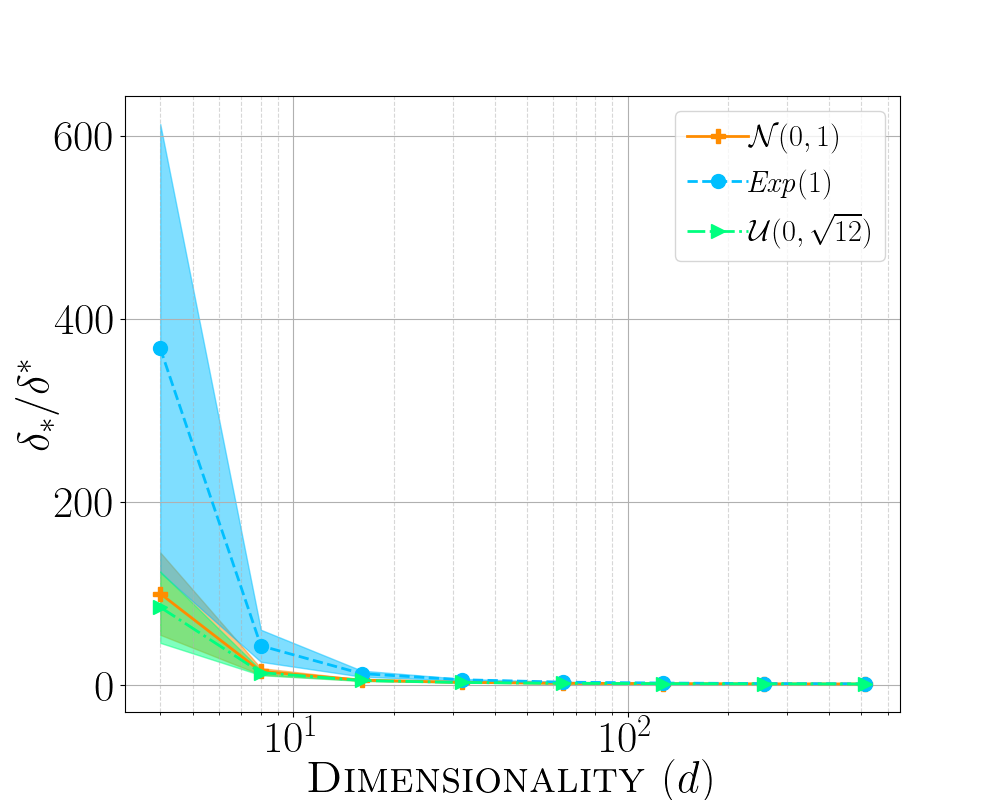
\includegraphics[width=0.52\linewidth]{figures/introduction-instability-ratio-l2.png}
    }\hspace*{-1.5em}
    \subfloat[\textsc{Percent Approximate Solutions}]{
        \label{figure:instability:instability:count}
        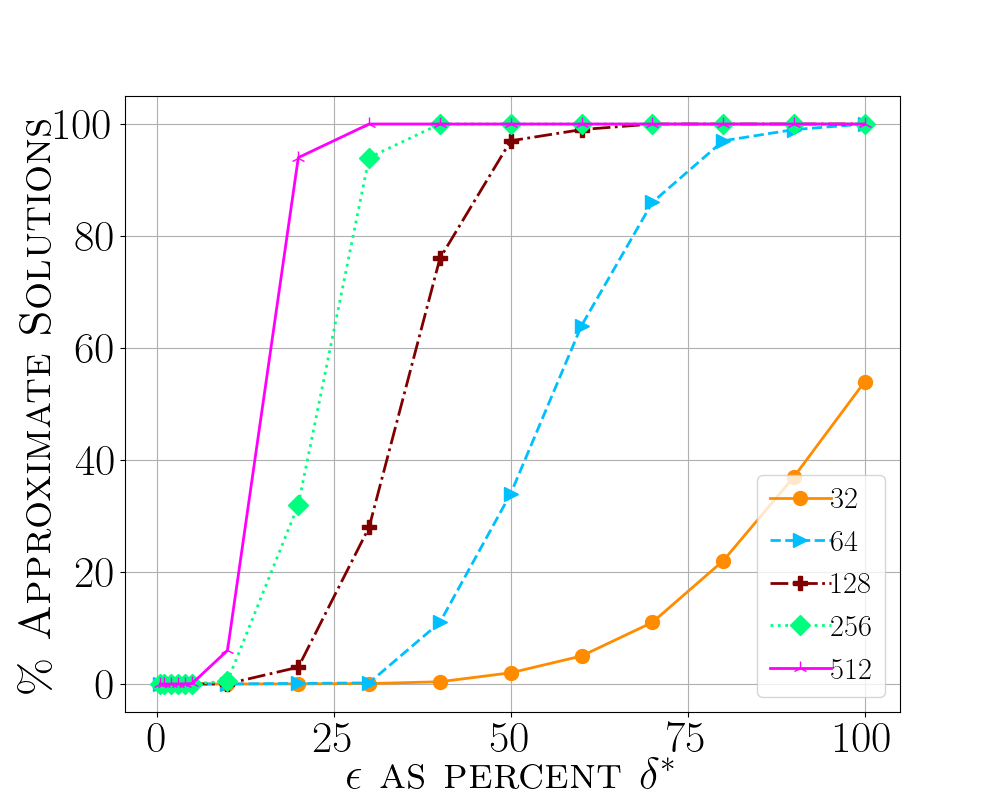
\includegraphics[width=0.52\linewidth]{figures/introduction-instability-count.png}
    }
    \caption{Simulation results for Theorem~\ref{theorem:instability:beyer} applied to NN with $L_2$ distance.
    \emph{Left}: The ratio between the maximum
    distance between a query and data points $\delta_\ast$, to the minimum distance $\delta^\ast$.
    The shaded region shows one standard deviation.
    As dimensionality increases, this ratio tends to $1$. \emph{Right}: The percentage of data points whose
    distance to a query is at most $(1 + \epsilon/100) \delta^\ast$, visualized for the Gaussian
    distribution---the trend is similar for other distributions. As $d$ increases, more vectors
    fall into the enlarged ball, making them valid solutions to the approximate NN problem.}
    \label{figure:instability:instability}
\end{figure}

Another way to understand this result is to count the number of data points that qualify
as approximate nearest neighbors. The theory predicts that, as $d$ increases, we can find a smaller
$\epsilon$ such that nearly all data points fall within $(1 + \epsilon) \delta^\ast$ distance from the query.
The results of our experiments confirm this phenomenon; we have plotted the results for the Gaussian distribution
in Figure~\subref*{figure:instability:instability:count}.

\subsection{Maximum Inner Product Search}

In the discussion above, we established that retrieval becomes unstable in
high dimensions if the data satisfies certain statistical conditions.
That meant that the difference between the maximum and the minimum distance
grows just as fast as the magnitude of the minimum distance, so that any approximate
solution becomes meaningless.

\begin{svgraybox}
The instability statement does not necessarily imply, however, that the distances
become small or converge to a certain value. But as we see in this section,
inner product in high dimensions does become smaller and smaller as a function of $d$.
\end{svgraybox}

The following theorem summarizes this phenomenon for a unit query point and bounded
data points.
Note that, the condition that $q$ is a unit vector is not restrictive in any way,
as the norm of the query point does not affect the retrieval outcome.

\begin{theorem}
    \label{theorem:instability:orthogonality-random-vectors}
    If $m$ data points with bounded norms,
    and a unit query vector $q$ are drawn \emph{iid}
    from a spherically symmetric\footnote{A distribution is spherically symmetric
    if it remains invariant under an orthogonal transformation.}
    distribution in $\mathbb{R}^d$, then:
    \begin{equation*}
        \lim_{d \rightarrow \infty} \probability\big[ \langle q, X \rangle > \epsilon \big] = 0.
    \end{equation*}
\end{theorem}
\begin{proof}
    By spherical symmetry, it is easy to see that $\ev[\langle q, X \rangle] = 0$.
    The variance of the inner product is then equal to $\ev[\langle q, X \rangle^2]$,
    which can be expanded as follows.
    
    First, find an orthogonal transformation $\Gamma: \mathbb{R}^d \rightarrow \mathbb{R}^d$ that maps
    the query point $q$ to the first standard basis (i.e., $e_1 = [1, 0, 0, \ldots, 0] \in \mathbb{R}^d$).
    Due to spherical symmetry, this transformation does not change the data distribution.
    Now, we can write:
    \begin{align*}
        \ev[\langle q, X \rangle^2] &= \ev[ \langle \Gamma q, \Gamma X \rangle^2] =
        \ev[(\Gamma X)_1^2] = \\
        &\ev[\frac{1}{d} \sum_{i=1}^d (\Gamma X)_i^2] = \frac{1}{d} \lVert X \rVert_2^2.
    \end{align*}
    In the above, the third equality is due to the fact that the distribution of the (transformed)
    vectors is the same in every direction. Because $\lVert X \rVert$ is bounded by assumption, the
    variance of the inner product between $q$ and a random data point tends to $0$ as $d \rightarrow \infty$.
    The claim follows.
\end{proof}

\begin{svgraybox}
The proof of Theorem~\ref{theorem:instability:orthogonality-random-vectors} tells us that
the variance of inner product grows as a function of $1/d$ and $\lVert X \rVert_2^2$.
So if our vectors have bounded norms, then we can find a $d$ such that inner products are
arbitrarily close to $0$. This is yet another reason that approximate MIPS could become meaningless.
But if our data points are clustered in (near) orthogonal subspaces, then approximate
MIPS over clusters makes sense---though, again, MIPS within clusters would be unstable.
\end{svgraybox}

\bibliographystyle{abbrvnat}
\bibliography{biblio}
